\section{Comparisons}
\label{sec:comparsisons}

In this section, a comparision between the ngspice and octave results is made. Moreover, we delve into the reasons regarding the diffences and similarities observed\\


\begin{figure} [!htb] 
  \minipage{0.9\textwidth}
  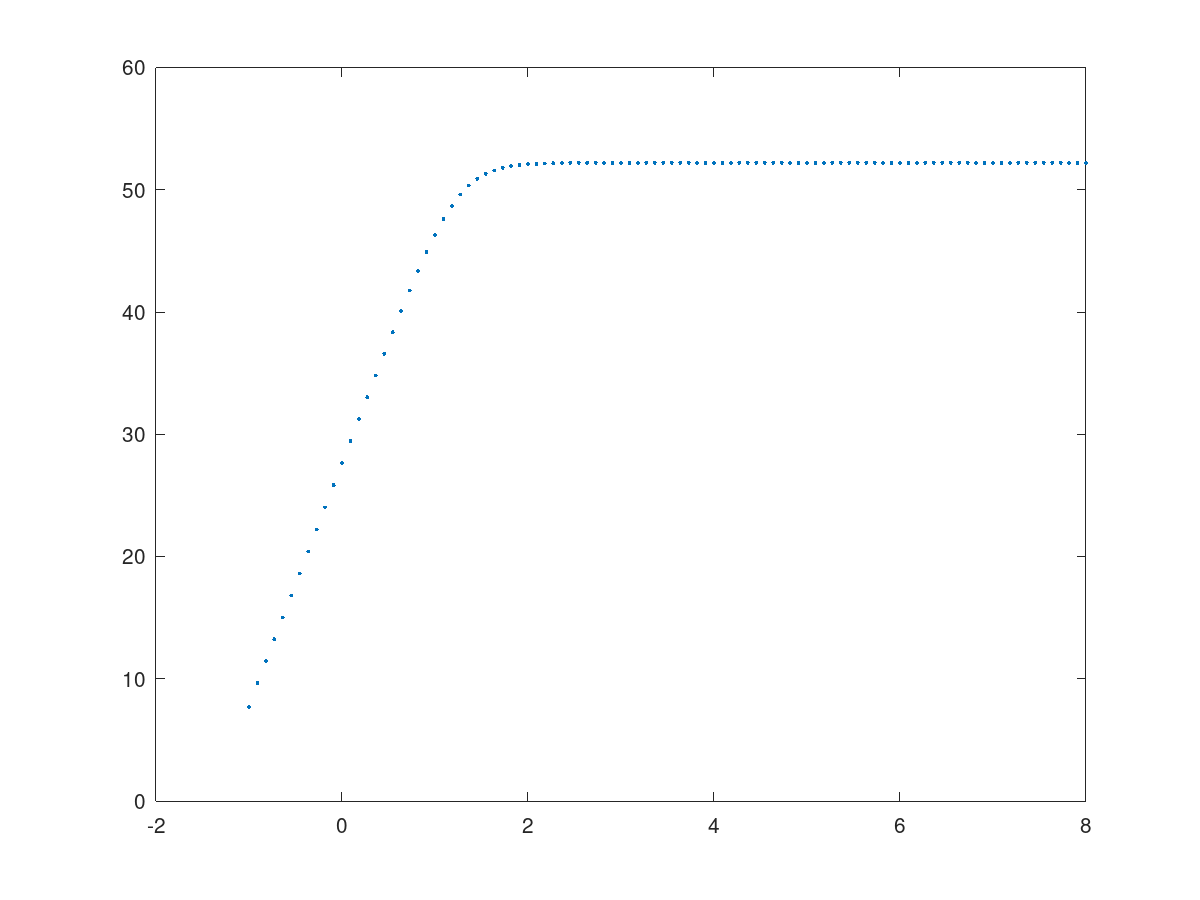
\includegraphics[width=\linewidth]{GAINVERDADEIRO.png}
  \caption{Amplifier circuit}
  \label{fig:theoplots}
  \endminipage\hfill
\end{figure}

%\begin{figure} [!htb] 
%  \minipage{0.9\textwidth}
%  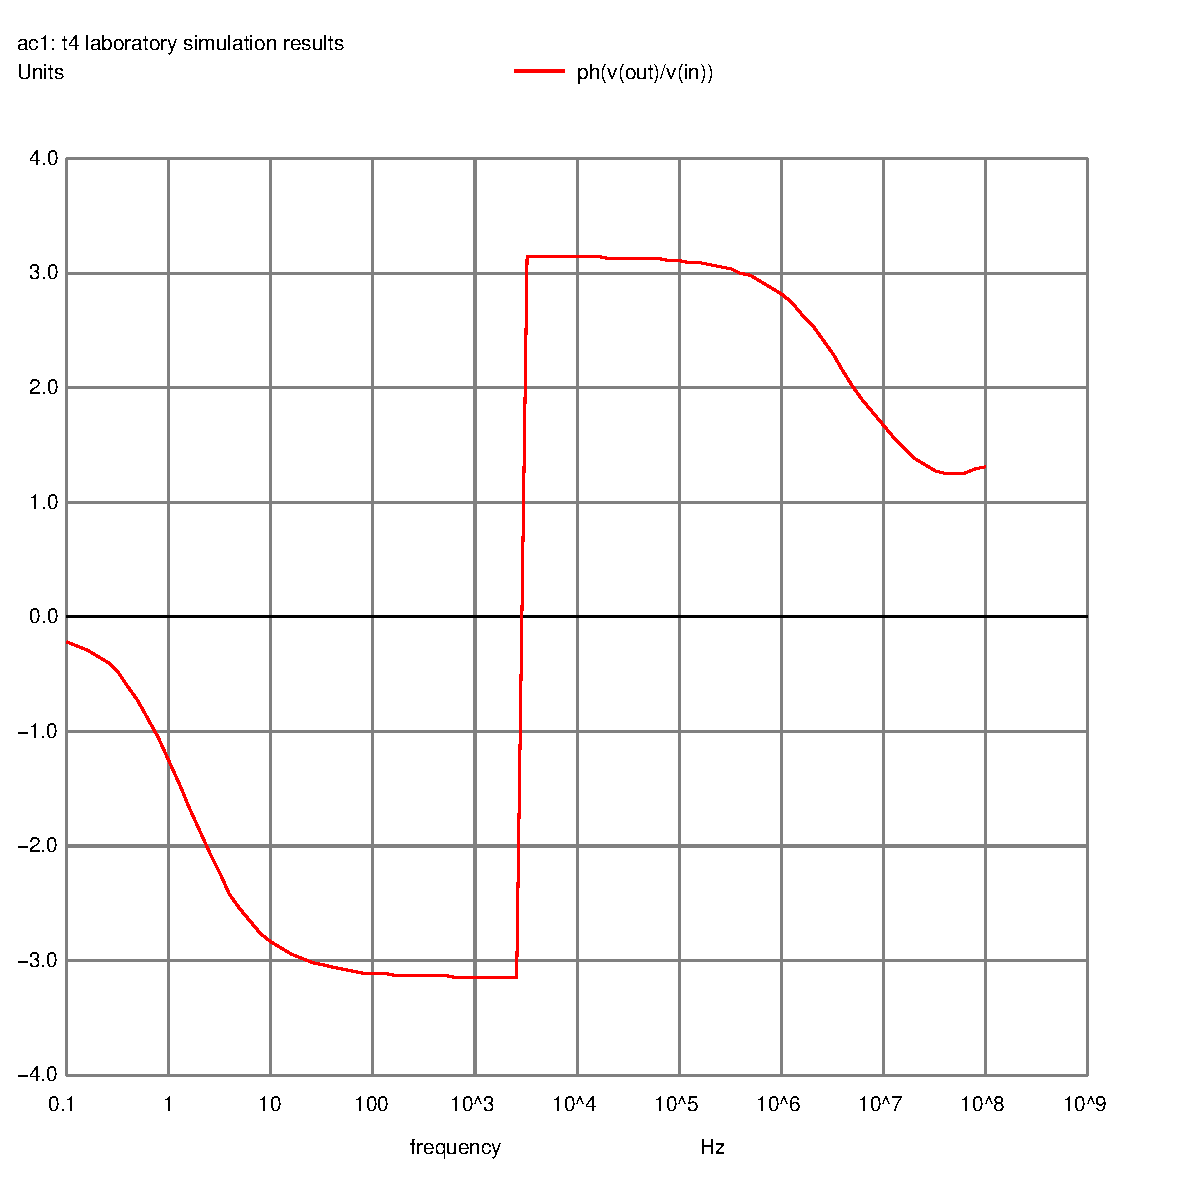
\includegraphics[width=\linewidth]{gain2.ps}
%  \caption{Amplifier circuit}
%  \label{fig:theoplots}
%  \endminipage\hfill
%\end{figure}




And now for the impedances values, in the tables down bellow we can compare side bye side:
\FloatBarrier
\begin{table}[h]
  \centering
  \begin{tabular}{|c|c|}
    \hline    
    zin & 2.738309e+00 \\ 

    \hline
  \end{tabular}
  \caption{Input Impedance by Ngspice}
  \label{tab:Spice1}
\end{table}
\FloatBarrier   

%\FloatBarrier
%\begin{table}[h]
%  \centering
%  \begin{tabular}{|c|}
%    \hline    
%    \input{output_tab.tex}
%    \hline
%  \end{tabular}
%  \caption{Output Impedance by Ngspice}
%  \label{tab:Spice1}
%\end{table}
%\FloatBarrier   

\FloatBarrier
\begin{table}[h]
  \centering
  \begin{tabular}{|c|c|}
    \hline    
    
 $Z_{in}$ & $Z_{out}$ \\ 
 115705 \$Omega   & 3.25315 \$Omega\\

    \hline
  \end{tabular}
  \caption{Input and Output Impedances by Octave}
  \label{tab:Spice1}
\end{table}
\FloatBarrier   


Comparing both results, we can that the gain is not the same. Such a disparity is visibly noticible for high frequencies, where the gain drops in the simulation, but stabilizes in the theoretical analysis. Such a result can be explain when one notices that gain was obtained by assuming a linear incremental model. This model is based on truncating the taylor series for each component, so that the circuit components can all have a linear dependency on frequency. However, such is an aproximation and, in this case, the error grows with the frequency, for transistors are non-linear devices that depend on it. By analysing the incremental model, one notes than only the capacitators present have a dependency on frequency, the transistor does not. Since the impendance of the capacitators will decrease with the rise in frequency, it eventually becomes negligible and the gain stabilizes.\\
It is also possible to see that the maximum gain is not the same, growing much quicker in the ngspice model, stabilizing at a lower frequency and at a higher value.\\
The impedances are 

% Aqui nesta parte discriminar os nossos valores referentes ao mérito do nosso trabalho.




